
% This LaTeX was auto-generated from MATLAB code.
% To make changes, update the MATLAB code and republish this document.

\documentclass{article}
\usepackage{graphicx}
\usepackage{color}

\sloppy
\definecolor{lightgray}{gray}{0.5}
\setlength{\parindent}{0pt}

\begin{document}

    
    
\subsection*{Contents}

\begin{itemize}
\setlength{\itemsep}{-1ex}
   \item Unknown Input Observer Dynamic System Matricies
   \item Construct the state space system
   \item Step one: Check rank
   \item Step two: Compute Observer Matricies
   \item Step three: check observability
   \item Pole Placement
   \item Finish observer design
   \item Simulation results
   \item Sim the system
   \item Plot the results
\end{itemize}


\subsection*{Unknown Input Observer Dynamic System Matricies}

\begin{par}
Sam Nazari April 2015 This example is form the book: Robust Model Based Fault Diagnosis for Dynamic Systems by J. Chen Please see the associated ShareLaTeX pdf file "UIO and Examples"
\end{par} \vspace{1em}
\begin{verbatim}
clear
clc
A = [-1 1 1;1 0 0;0 1 -1];
B = [1;0;1];
C = [1 0 0;0 1 0]; % this is the orginal system that shafai proposed, but
%I am changing it to make the pair A1,C observable
%C = [1 0 1;0 1 0];
D = 0;
E = [1;0;0];
\end{verbatim}


\subsection*{Construct the state space system}

\begin{par}
Let us construct the system as a state space object for simulation.
\end{par} \vspace{1em}
\begin{verbatim}
sys = ss(A,B,C,D);
\end{verbatim}


\subsection*{Step one: Check rank}

\begin{par}
We check to see if the rank(CE) = rank(E) = 1
\end{par} \vspace{1em}
\begin{verbatim}
rank(C*E)
rank(E)
\end{verbatim}

        \color{lightgray} \begin{verbatim}
ans =

     1


ans =

     1

\end{verbatim} \color{black}
    

\subsection*{Step two: Compute Observer Matricies}

\begin{par}
Since we have no issues in the previous step, let us compute the observer matrices now:
\end{par} \vspace{1em}
\begin{verbatim}
H = E*inv((C*E)'*(C*E))*(C*E)'
T = eye(3)-H*C
A1 = T*A
\end{verbatim}

        \color{lightgray} \begin{verbatim}
H =

     1     0
     0     0
     0     0


T =

     0     0     0
     0     1     0
     0     0     1


A1 =

     0     0     0
     1     0     0
     0     1    -1

\end{verbatim} \color{black}
    

\subsection*{Step three: check observability}

\begin{par}
We must check the system A1,C observability
\end{par} \vspace{1em}
\begin{verbatim}
rank(obsv(A1,C))
% Since rank(obsv(A1,C))<n, the pair (A1,C) is not observable.  Let us
% utilize the PBH test to see which eigenvalue of A1 is the culprit.
l = eig(A1);
lam1=l(1),lam2=l(2),lam3=l(3)
plam1 = rank([lam1*eye(3)-A1;C])
plam2 = rank([lam2*eye(3)-A1;C])
plam3 = rank([lam3*eye(3)-A1;C])
% it can be seen that the eigenvalue that fails the PBH test is already in
% the left half plane (at -1).  Therefore, the pair (A1,C) is detectible
% and a UIO exists.
\end{verbatim}

        \color{lightgray} \begin{verbatim}
ans =

     2


lam1 =

    -1


lam2 =

     0


lam3 =

     0


plam1 =

     2


plam2 =

     3


plam3 =

     3

\end{verbatim} \color{black}
    

\subsection*{Pole Placement}

\begin{par}
Pole placement is used to assign the observer poles
\end{par} \vspace{1em}
\begin{verbatim}
K1 = [3 0;-1 2;-1/2 0]
\end{verbatim}

        \color{lightgray} \begin{verbatim}
K1 =

    3.0000         0
   -1.0000    2.0000
   -0.5000         0

\end{verbatim} \color{black}
    

\subsection*{Finish observer design}

\begin{par}
Finally, the F and K matricies are computed
\end{par} \vspace{1em}
\begin{verbatim}
F = A1-K1*C
K = K1 + F*H
eig(F)
\end{verbatim}

        \color{lightgray} \begin{verbatim}
F =

   -3.0000         0         0
    2.0000   -2.0000         0
    0.5000    1.0000   -1.0000


K =

     0     0
     1     2
     0     0


ans =

    -1
    -2
    -3

\end{verbatim} \color{black}
    

\subsection*{Simulation results}

\begin{par}
Set up simulation initial condiditons
\end{par} \vspace{1em}
\begin{verbatim}
x1_0 = 1;
x2_0 = 0;
x3_0 = 0;

d = 10;
TSIM = 50;
\end{verbatim}


\subsection*{Sim the system}

\begin{verbatim}
sim('shafExPosSys')
\end{verbatim}

        \color{lightgray} \begin{verbatim}Warning: Input port 1 of 'shafExPosSys/UIO' is not connected. 
Warning: Input port 1 of 'shafExPosSys/dynamics' is not connected. 
\end{verbatim} \color{black}
    

\subsection*{Plot the results}

\begin{verbatim}
figure(1)
plot(tout,Xerr(:,1),'b'),hold on
plot(tout,Xerr(:,2),'g'),hold on
plot(tout,Xerr(:,3),'r')
xlabel('Time in seconds'),ylabel('State Estimate Error')
title('Positive Dynamic System and Positive UIO Observer State Estimation Error')
legend('x_1','x_2','x_3')
\end{verbatim}

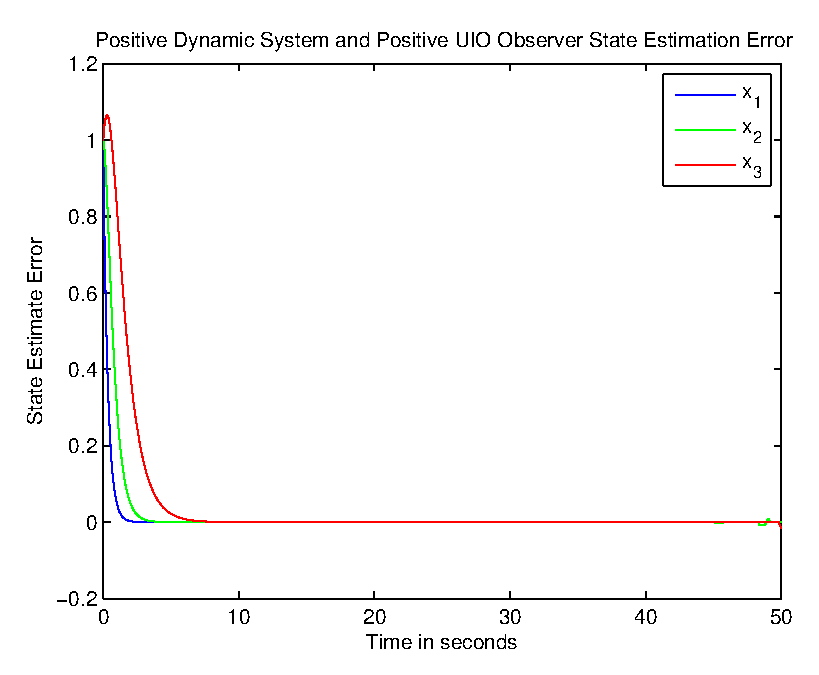
\includegraphics [width=4in]{shafaiExPosSys_01.eps}



\end{document}
    
